\section{Introduction}

% \note{jk: you need two paragraphs in intro to describe the problem statement.
% 	What I read in the first paragraph is not relevant with the problem that your
% 	thesis solves. The problem is: 1. Data analytics and search engines running on JVM need large heaps.
% 	2. A promising solution for large heaps that do not increase the GC cost is dual-heap designes, such as TeraHeap. Explain how does TeraHeap work and explain the problem of DRAM division.
% 	3. Then put a paragraph describing in high level your solution and how does this solution work.
% 	4. write where you implement your solution and provide some high-level results.
% }


Data analytics and search engines such as \textbf{Apache Lucene}
\cite{klinaftakis2025thesis} and \textbf{Apache Spark} require large heaps in order 
to be able to store the required data for execution. Moreover, Lucene performs intensive indexing and query
evaluation on large in-memory data structures such as a query cache, while
Spark continuously allocates and frees large volumes of temporary objects
during distributed computation. Both systems report highly dynamic memory
behavior, exibiting phases of increased GC pressure.

A solution for large heaps that does not add overheads to the GC cost is dual-heap designs.
In this thesis we use TeraHeap, the G1 intergated version, which, is a
tiered memory management system. TeraHeap's implementation
provides the option of the H1 heap which is managed by the JVM's Garbage Collector and the secondary H2 heap, which is
backed by a memory-mapped file and accessed through the operating system's page cache, for cold or less frequently accessed objects. 
The DRAM division between the main heap and the pagecache must happen at the beginning of an execution statically, which
presents a problem since the system can not adapt in phases with different memory and I/O demands. 

Moreover, Figure~\ref{fig:vanilla-dram-underutilization} illustrates a native
Lucene benchmark using a total of 8GB of DRAM, evenly split between H1 and the
OS page cache. At the beginning of the run, the heap usage rapidly spikes,
indicating that an increased number of GC cycles is occurring. As the benchmark execution progresses, the heap usage
stabilizes at a much lower level, suggesting that part the heap could be shrunk 
and the page increased to hold more data from the H2 file, without massively affecting GC
performance. This behavior highlights the limitations of static partitioning.
\begin{figure}[htbp]
	\centering
	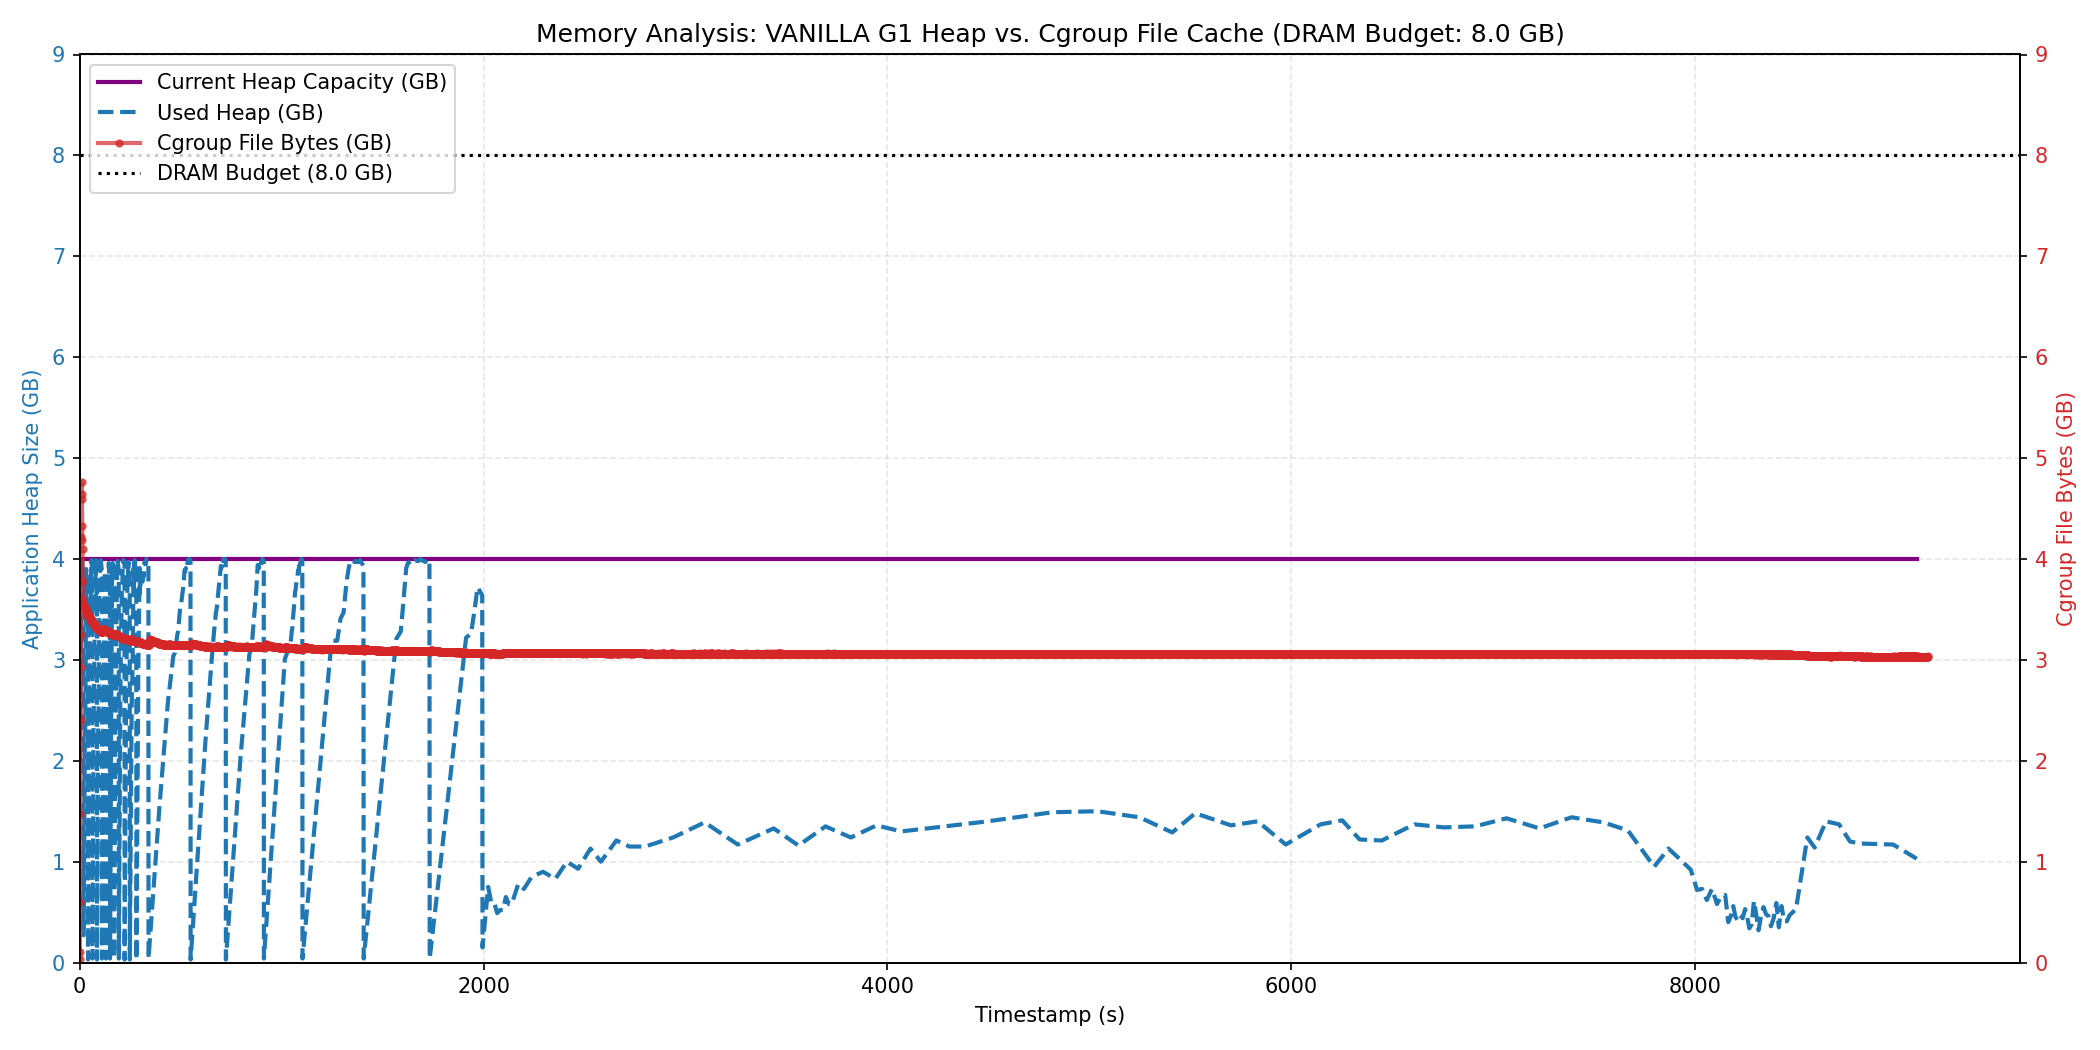
\includegraphics[width=1\linewidth]{fig/combined_memory_timeline_vanilla_g1.png}
	\caption{
		M1 Lucene benchmark with static DRAM configuration of 4GB H1 and 4GB pagecache.
	}
	\label{fig:vanilla-dram-underutilization}
\end{figure}

To address this limitation, we port \textbf{FlexHeap} to our system,
a dynamic resizing policy that operates at runtime by
dividing execution into sampling intervals. During each interval, it tracks the
number of CPU cycles lost to GC (garbage collection) and the I/O overheads including I/O caused by
accesses to the (H2) memory-mapped file. At the end of each interval, it compares the percent 
change between the two metrics, relative to the previous intervals. If garbage
collection overhead has increased more than I/O stalls, FlexHeap signals G1 to grow
the H1 heap to relieve GC pressure. Inversely, if I/O delays have increased,
a shrink heap action is invoked, shifting the remaining memory towards the pagecache, via cgroups, to reduce evictions and hold 
more data from the H2 file. Across Lucene's and Spark's benchmarks, FlexHeap reports execution time improvements
up to 70\% and 9\% accordingly.



